%% ── Section 5: Results and Discussion ───────────────────────
\section{Results and Discussion}
\label{sec:results}

\subsection{Overall Performance}

Table~\ref{tab:results} gives the test QWK of each method at its best validation
round, averaged over three seeds. The federated methods score between 0.640 and
0.681, close to the 0.682 of the centralised model. On the IID and real-site
partitions, the methods differ by at most 0.01, which is within the variation
between seeds. Under $\alpha=0.1$, FedProx scores highest (0.664) and OrdinalFed
lowest (0.640). This table hides what happens in the other rounds, because the
reported round is chosen on the validation split. For FedAvg under $\alpha=0.1$,
for example, the best validation round is always the first one, before the
collapse.

\begin{table}[t]
\caption{Test QWK at the Best Validation Round (Mean $\pm$ Std over Three Seeds).
Bold: Best Federated Method per Column.}
\label{tab:results}
\centering
\footnotesize
\setlength{\tabcolsep}{4pt}
\begin{tabular}{@{}lccc@{}}
\toprule
\textbf{Method} & \textbf{IID} & \textbf{Dirichlet ($\alpha=0.1$)} & \textbf{Real-Site} \\
\midrule
Centralised (reference) & 0.682 & 0.682 & 0.682 \\
\midrule
FedAvg~\cite{mcmahan2017fedavg}   & 0.677\sd{.008} & 0.647\sd{.010} & 0.673\sd{.004} \\
FedProx~\cite{li2020fedprox}      & \textbf{0.681}\sd{.014} & \textbf{0.664}\sd{.015} & 0.671\sd{.005} \\
AccWt                             & --             & 0.651\sd{.011} & \textbf{0.674}\sd{.009} \\
OrdinalFed                        & 0.679\sd{.006} & 0.640\sd{.007} & 0.666\sd{.002} \\
OrdinalFed + Prox                 & --             & 0.659\sd{.012} & 0.672\sd{.007} \\
\bottomrule
\end{tabular}
\end{table}

\subsection{Stability Under Extreme Skew}

Fig.~\ref{fig:qwk_curves} shows the test QWK of the global model after every round,
with one panel per partition. Lines show the mean over three seeds, shaded bands
$\pm$ one standard deviation, and the dashed line the test QWK of the centralised
model. On the IID and real-site partitions, all three methods stay close to the
centralised line. Under $\alpha=0.1$, FedAvg collapses from round~5 onwards, FedProx
stays flat, and OrdinalFed avoids the collapse but goes up and down from round to
round.

%% FULL-WIDTH FIGURE: QWK trajectories
%% (placed after its description — Reviewer #3, comments 3 and 6)
\begin{figure*}[t]
  \centering
  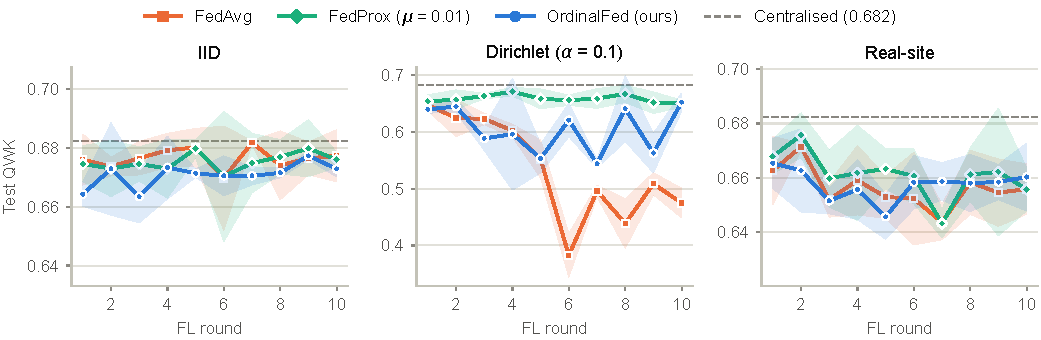
\includegraphics[width=\textwidth]{fig4_qwk_combined.pdf}
  \caption{\normalsize Test QWK of the global model after each of the 10 rounds for
  the IID, Dirichlet ($\alpha=0.1$) and real-site partitions (mean $\pm$ std over
  three seeds). Under $\alpha=0.1$, FedAvg collapses, OrdinalFed avoids the
  collapse but fluctuates, and FedProx stays stable.}
  \label{fig:qwk_curves}
\end{figure*}

Table~\ref{tab:stability} summarises the ten rounds under $\alpha=0.1$. Compared
with FedAvg, OrdinalFed raises the worst round from 0.378 to 0.514 and the mean over
rounds from 0.535 to 0.604, with no change at the hospitals. FedProx, which changes
local training instead, is the most stable method (worst round 0.641). Adding
FedProx's proximal term to OrdinalFed brings it close to FedProx (worst round 0.627)
and gives the best final round (0.664), but it is not more stable than FedProx
alone.

\begin{table}[t]
\caption{Test QWK Across the 10 Rounds Under Dirichlet Skew ($\alpha=0.1$):
Mean over Rounds, Worst Round and Final Round. Bold: Best per Column.}
\label{tab:stability}
\centering
\footnotesize
\setlength{\tabcolsep}{4pt}
\begin{tabular}{@{}lccc@{}}
\toprule
\textbf{Method} & \textbf{Mean} & \textbf{Worst} & \textbf{Final} \\
\midrule
FedAvg            & 0.535\sd{.004} & 0.378\sd{.035} & 0.475\sd{.026} \\
FedProx           & \textbf{0.659}\sd{.003} & \textbf{0.641}\sd{.008} & 0.650\sd{.006} \\
AccWt             & 0.627\sd{.011} & 0.571\sd{.017} & 0.657\sd{.018} \\
OrdinalFed        & 0.604\sd{.005} & 0.514\sd{.027} & 0.652\sd{.016} \\
OrdinalFed + Prox & 0.651\sd{.003} & 0.627\sd{.005} & \textbf{0.664}\sd{.013} \\
\bottomrule
\end{tabular}
\end{table}

\subsection{What Makes the Aggregation Stable?}

Table~\ref{tab:ablation} separates the two parts. OrdinalLoss alone does not stop
the collapse: with image-count weights, its worst round (0.380) is the same as
FedAvg's. QWK-weighted aggregation with cross-entropy raises the worst round to
0.586, but giving every client the same weight raises it further, to 0.630. Scoring
clients by accuracy instead of QWK (AccWt, Table~\ref{tab:stability}) gives almost
the same result as scoring them by QWK (worst round 0.571 versus 0.586).

The logged aggregation weights explain this. Under $\alpha=0.1$, the two smallest
clients hold 5.9\% of the images, so FedAvg gives them 5.9\% of the weight. The
quality weights of Eq.~\eqref{eq:quality} are close to equal, so OrdinalFed raises
their combined weight from 23.5\% in round~1 to 40.8\% in round~10. The QWK scores
themselves carry little information at this scale. A client's score on the
50-image set $\mathcal{V}$ changes by 0.13 on average from one round to the next,
and in round~10 the largest quality weight is only 1.19 times the smallest. The
stability therefore comes from moving weight towards small clients, not from the
QWK scores. OrdinalLoss lowers performance slightly in both comparisons.

The lower block of Table~\ref{tab:ablation} tests three settings of OrdinalFed,
each fixed before the runs and compared on mean validation QWK. All three do
better than the default. Sharper quality weights ($\tau=0.5$) score best (0.795
versus 0.761), closely followed by using quality weights from the first round
($\beta_0=0$, 0.793). Both still score below equal weighting (0.810) and FedProx
(0.808).

\begin{table}[t]
\caption{Contribution of Each Component and Setting Under $\alpha=0.1$. Mean: QWK
Averaged over the 10 Rounds; Worst: Lowest Round. CE: Class-Weighted Cross-Entropy.
Default: $\lambda=0.5$, $\beta_0=0.5$, $\tau=3$.}
\label{tab:ablation}
\centering
\footnotesize
\setlength{\tabcolsep}{3pt}
\begin{tabular}{@{}lccc@{}}
\toprule
\textbf{Configuration} & \textbf{Mean val} & \textbf{Mean test} & \textbf{Worst test} \\
\midrule
CE + image-count weights (FedAvg) & 0.670\sd{.011} & 0.535\sd{.004} & 0.378\sd{.035} \\
OrdinalLoss + image-count weights & 0.659\sd{.015} & 0.522\sd{.011} & 0.380\sd{.018} \\
CE + QWK weights                  & 0.786\sd{.006} & 0.633\sd{.010} & 0.586\sd{.006} \\
CE + equal weights                & \textbf{0.810}\sd{.007} & \textbf{0.658}\sd{.006} & \textbf{0.630}\sd{.021} \\
\midrule
OrdinalFed (default)      & 0.761\sd{.003} & 0.604\sd{.005} & 0.514\sd{.027} \\
\quad with $\lambda=0.1$  & 0.776\sd{.007} & 0.622\sd{.006} & 0.571\sd{.019} \\
\quad with $\beta_0=0$    & 0.793\sd{.005} & 0.631\sd{.009} & 0.571\sd{.011} \\
\quad with $\tau=0.5$     & 0.795\sd{.006} & 0.637\sd{.005} & 0.592\sd{.009} \\
\bottomrule
\end{tabular}
\end{table}

\subsection{Class-Wise Performance}

Table~\ref{tab:pergrade} gives the per-grade recall and F1 on the test split. All
methods find Grade~0 reliably (recall $\geq 0.95$) but almost never find Grade~1
(recall $\leq 0.05$), which makes up only 5\% of the training set. Grade~2 recall
stays near 0.4 because many test Grade~2 images are predicted as Grade~0
(Sec.~\ref{sec:limitations}). OrdinalFed has the highest Grade~3 recall in both
partitions (0.36 versus 0.27--0.31 under $\alpha=0.1$, and 0.40 versus 0.35--0.38
on the real-site partition). This is a modest gain on the rarest severe grade. For
Grade~4, the three methods are within 0.05 of each other.

\begin{table}[t]
\caption{Per-Grade Recall / F1 on the Test Split at the Best Validation Round
(Mean over Three Seeds).}
\label{tab:pergrade}
\centering
\footnotesize
\setlength{\tabcolsep}{2.5pt}
\begin{tabular}{@{}lccccc@{}}
\toprule
\textbf{Method} & \textbf{G0} & \textbf{G1} & \textbf{G2} & \textbf{G3} & \textbf{G4} \\
\midrule
\multicolumn{6}{@{}l}{\textit{Dirichlet ($\alpha=0.1$)}} \\
FedAvg     & .96/.80 & .05/.07 & .41/.52 & .27/.32 & .66/.73 \\
FedProx    & .95/.81 & .05/.06 & .43/.54 & .31/.34 & .69/.74 \\
OrdinalFed & .97/.80 & .04/.07 & .39/.50 & .36/.38 & .64/.73 \\
\midrule
\multicolumn{6}{@{}l}{\textit{Real-site}} \\
FedAvg     & .98/.81 & .04/.06 & .44/.55 & .35/.37 & .66/.73 \\
FedProx    & .98/.81 & .04/.06 & .43/.54 & .38/.38 & .65/.73 \\
OrdinalFed & .97/.81 & .04/.06 & .43/.54 & .40/.38 & .64/.73 \\
\bottomrule
\end{tabular}
\end{table}

\subsection{Communication and Computational Overhead}

OrdinalFed sends the same model weights as FedAvg, so it adds no communication.
Once per round, the server evaluates each of the $K$ client models on the 50 images
of $\mathcal{V}$. This took a median of 1.2~s per round for $K=5$ on an Intel Arc
B580 GPU, about 0.6\% of the 195~s a full round takes.

\subsection{Limitations}
\label{sec:limitations}

Grade~1 recall stays at or below 0.05 for every method (Table~\ref{tab:pergrade}).
All models also score lower on the DDR test split than on the validation split. The
centralised model drops from a QWK of 0.834 to 0.682, and the federated models drop
by a similar amount. Most of this drop comes from Grade~2 images predicted as
Grade~0 (about 45\% of test Grade~2 images, against about 12\% on the validation
split), and the test split has a different mix of camera resolutions. Validation
QWK therefore overestimates performance on new images, which is why all main
results are reported on the test split. The 50-image server set $\mathcal{V}$ is too
small to rank clients reliably, which limits the value of QWK-based weighting, and
it needs labelled images on the server. Finally, all results come from one dataset
at $224 \times 224$ resolution with five clients. Larger server sets, higher
resolution and more clients are left for future work.
